\documentclass{article}

\usepackage{listings}
\usepackage{minted}
\usepackage{titlesec}
\usepackage{graphicx}
\usepackage{float}
\usepackage{mdframed}
\usepackage{xcolor}
\usepackage{xurl}
\usepackage{geometry}

\newgeometry{hmargin={17mm,17mm}}

% Prevent word break at end of line
\tolerance=1
\emergencystretch=\maxdimen
\hyphenpenalty=10000
\hbadness=10000

\title{Evaluation task for Awkward Array GSoC project}
\author{Pratyush Das$^1$}
% https://tex.stackexchange.com/a/315873/193728
\date{%
    $^1$Institute of Engineering \& Management, Kolkata\\%
}

\begin{document}

\definecolor{light-gray}{gray}{0.95}

\maketitle

\begin{abstract}

    In this report, we demonstrate a sample GPU kernel designed to be an alternative to the CPU backend for array operations in the Awkward Array project. In particular, we implement a CUDA translation of the \textit{awkward\_listarray\_compact\_offsets} CPU kernel, and show how parallelizing the code on a GPU could significantly increase the speed of computation. The motivation of this report is to serve as an evaluation task to qualify to work on the project titled ``Awkward Array GPU kernels" under the mentorship of Jim Pivarski and David Lange.

\end{abstract}

\section{Introduction}

The sample CPU kernel (directly taken from the Awkward Array codebase) to be translated is defined below -
\begin{mdframed}[backgroundcolor=light-gray, roundcorner=10pt,leftmargin=0.5, rightmargin=0.5, innertopmargin=1,innerbottommargin=1, outerlinewidth=1, linecolor=light-gray]
\lstinputlisting[breaklines]{Code/cpukernel.c}
\end{mdframed}
Translating this particular CPU kernel serves as a good test because parallelizing this CPU kernel involves overcoming the loop carried dependency in the above code -
\begin{mdframed}[backgroundcolor=light-gray, roundcorner=10pt,leftmargin=0.5, rightmargin=0.5, innertopmargin=1,innerbottommargin=1, outerlinewidth=1, linecolor=light-gray]
\begin{lstlisting}
tooffsets[i + 1] = tooffsets[i] + (stop - start);
\end{lstlisting}
\end{mdframed}
where \mintinline{c}{tooffsets[i + 1]} depends on \mintinline{c}{toffsets[i]}.\\

The above algorithm can be visualized to illustrate its linear nature -
\begin{figure}[H]
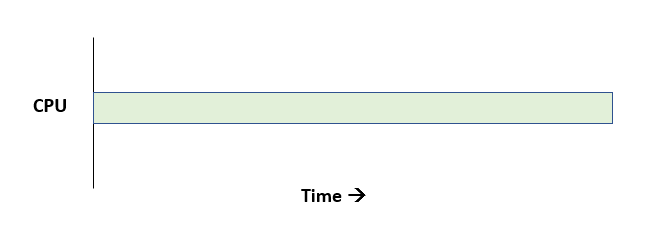
\includegraphics[width=\textwidth]{Graphics/cpu.PNG}
\caption{Visualizing sequential CPU algorithm}
\end{figure}

\subsection{Implementation of GPU algorithm}

The evaluation task required creating a parallel algorithm as an alternative for the sequential CPU algorithm. There are several ways to do this -
\begin{enumerate}
\item OpenCL, which is a more uniform interface to write parallel algorithms to be executed on multiple backends, but is slower than CUDA and losing popularity.
\item CUDA, which is an easier and more performant interface for executing parallel algorithms only on an NVIDIA GPU.
\end{enumerate}
Due to the availability of an NVIDIA GPU and performance requirements, we have decided to use CUDA to write and execute our parallel algorithms.
\smallbreak
\noindent We use some CUDA intrinsics like \mintinline{c}{thrust} in our sample code for the evaluation task which we might not use in the production code due to avoid locking the implementation to CUDA and allow expansion to newer interfaces in the future.

\section{Sequential algorithm on an Nvidia GPU}

\subsection{Sequential algorithm on a single thread}

\begin{figure}[H]
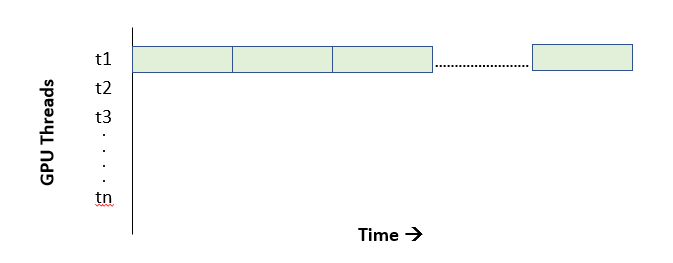
\includegraphics[width=\textwidth]{Graphics/naivesingle.PNG}
\caption{Visualizing GPU threads at work}
\end{figure}
\begin{mdframed}[backgroundcolor=light-gray, roundcorner=10pt,leftmargin=0.5, rightmargin=0.5, innertopmargin=1,innerbottommargin=1, outerlinewidth=1, linecolor=light-gray]
\lstinputlisting[breaklines]{Code/naivesinglefunc.cu}
\end{mdframed}
In the above code block\footnote{Full benchmarking code: \url{https://github.com/reikdas/GSoC-Proposal-2020/blob/master/testgsoc/naivesingle.cu}} we execute the algorithm only for a single GPU thread while the other threads sit idle.
\begin{mdframed}[backgroundcolor=light-gray, roundcorner=10pt,leftmargin=0.5, rightmargin=0.5, innertopmargin=1,innerbottommargin=1, outerlinewidth=1, linecolor=light-gray]
\begin{lstlisting}
    if (idx == 0) {
        ...
    }
\end{lstlisting}
\end{mdframed}
where the variable \mintinline{c}{idx} is the thread index.\\
\\
Since CUDA GPU kernels have to be of the return type void, we use additional device functions, \mintinline{c}{success_cuda} and \mintinline{c}{failure_cuda} to record whether the kernel behaved as expected.\\
\begin{mdframed}[backgroundcolor=light-gray, roundcorner=10pt,leftmargin=0.5, rightmargin=0.5, innertopmargin=1,innerbottommargin=1, outerlinewidth=1, linecolor=light-gray]
\begin{lstlisting}
__device__
void success_cuda(Error* err) {
  err.str = nullptr;
  err.identity = kSliceNone;
  err.attempt = kSliceNone;
  err.extra = 0;
}

__device__
void failure_cuda(const char* str, int64_t identity, 
                  int64_t attempt, Error* err) {
  err.str = str;
  err.identity = identity;
  err.attempt = attempt;
  err.extra = 0;
}
\end{lstlisting}
\end{mdframed}
We use a flag implemented using shared memory and the CUDA intrinsic thread synchronization 
\begin{mdframed}[backgroundcolor=light-gray, roundcorner=10pt,leftmargin=0.5, rightmargin=0.5, innertopmargin=1,innerbottommargin=1, outerlinewidth=1, linecolor=light-gray]
\begin{lstlisting}
    __shared__ int flag[1];
    ...
    __syncthreads();
    if (flag[0] != 1) {
        ...
    }
\end{lstlisting}
\end{mdframed}
to determine whether the \mintinline{c}{success_cuda()} call should be executed once the \mintinline{c}{failure_cuda()} call has already been reached by one of the GPU threads.

\subsection{Sequential algorithm on multiple threads}

\begin{figure}[H]
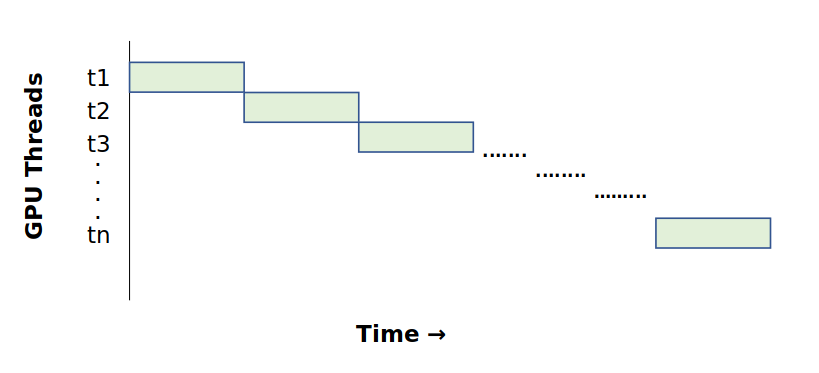
\includegraphics[width=\textwidth]{Graphics/naivemulti.PNG}
\caption{Visualizing GPU threads at work}
\end{figure}
\begin{mdframed}[backgroundcolor=light-gray, roundcorner=10pt,leftmargin=0.5, rightmargin=0.5, innertopmargin=1,innerbottommargin=1, outerlinewidth=1, linecolor=light-gray]
\lstinputlisting[breaklines]{Code/naivemultifunc.cu}
\end{mdframed}
The sequential algorithm on multiple GPU threads implementation above\footnote{Full benchmarking code: \url{https://github.com/reikdas/GSoC-Proposal-2020/blob/master/testgsoc/naivemultiblocks.cu}} differs only slightly from the sequential algorithm on single GPU threads implementation.
\smallbreak
\noindent The main difference is that the multiple GPU threads implementation has all the threads execute the algorithm one after another, instead of all at the same time. When one thread is being executed, the other threads sit idly, then the next thread is executed while the previous and all other threads sit idle.
\begin{mdframed}[backgroundcolor=light-gray, roundcorner=10pt,leftmargin=0.5, rightmargin=0.5, innertopmargin=1,innerbottommargin=1, outerlinewidth=1, linecolor=light-gray]
\begin{lstlisting}
    _for (int i = 0; i < length; i++) {
      ...
      if (i == idx) {
        ... 
        }
    }
\end{lstlisting}
\end{mdframed}
We use the CUDA intrinsic \mintinline{c}{__syncthreads()} before each iteration of the loop to ensure that all the threads are at the same position and ready to be executed before each thread is executed.

\section{Parallel algorithm on an Nvidia GPU}

\begin{figure}[H]
\hfill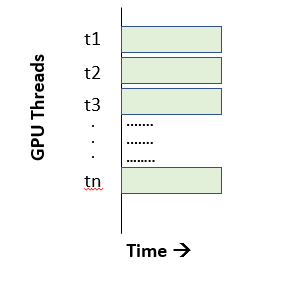
\includegraphics[scale=0.72]{Graphics/gpu.PNG}\hspace*{\fill}
\caption{Visualizing GPU threads at work}
\end{figure}
\begin{mdframed}[backgroundcolor=light-gray, roundcorner=10pt,leftmargin=0.5, rightmargin=0.5, innertopmargin=1,innerbottommargin=1, outerlinewidth=1, linecolor=light-gray]
\lstinputlisting[breaklines]{Code/thrustfunc.cu}
\end{mdframed}
The above code\footnote{Full benchmarking code: \url{https://github.com/reikdas/GSoC-Proposal-2020/blob/master/testgsoc/thrust.cu}}

\section{Benchmarks}
We have compared the performance of the various algorithms relative to each other\footnote{Benchmarking numbers: \url{https://github.com/reikdas/GSoC-Proposal-2020/blob/master/testgsoc/data.txt} generated using \url{https://github.com/reikdas/GSoC-Proposal-2020/blob/master/testgsoc/plotter.py}}.
\begin{figure}[H]
\hfill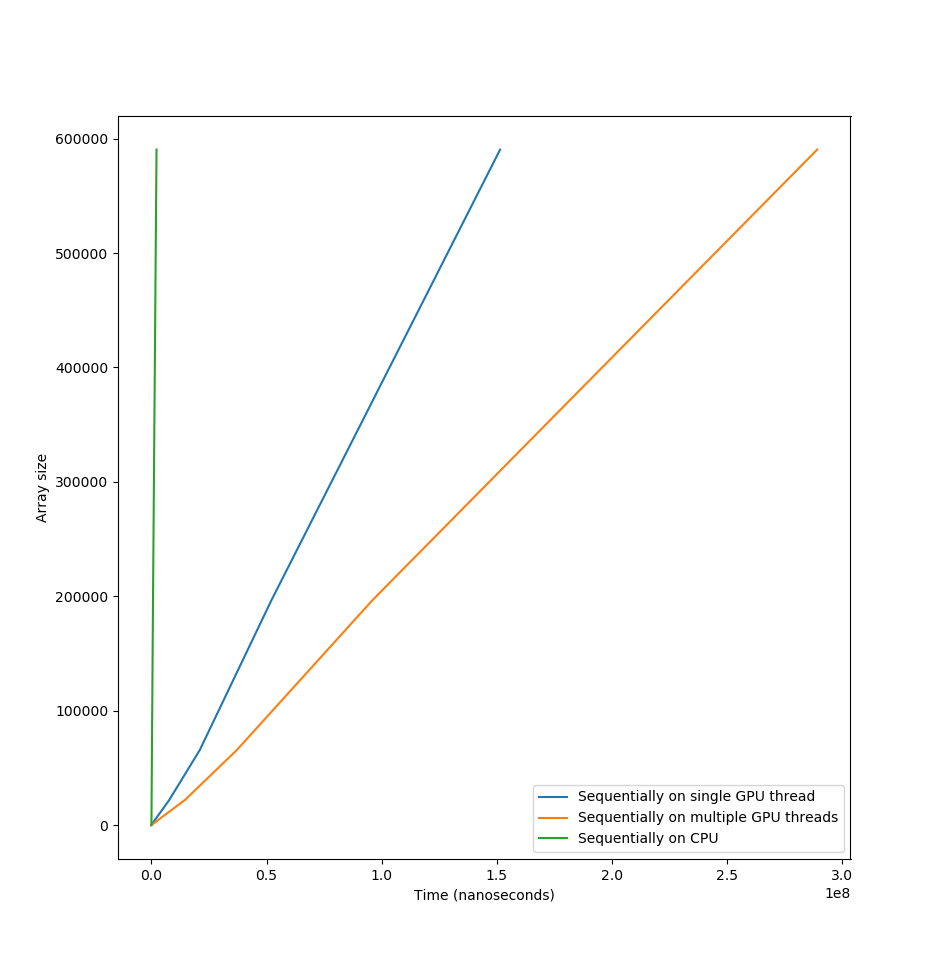
\includegraphics[scale=0.5]{Graphics/naivegpucpu.png}\hspace*{\fill}
\caption{Comparing performance of sequential GPU algorithms with CPU algorithm}
\end{figure}
We can see that the sequential algorithms on the GPU run much slower than the sequential algorithm on the CPU. This can be attributed to the inherent difference in the design of GPUs and CPUs. GPUs are designed to operate on independent data in parallel, whereas CPUs are optimized to execute a single stream of instructions as quickly as possible. So when we are executing a single instruction stream on the GPU, it is expected that the time for completion will be more than the time for completion of the same instructions on a CPU.

\begin{figure}[H]
\hfill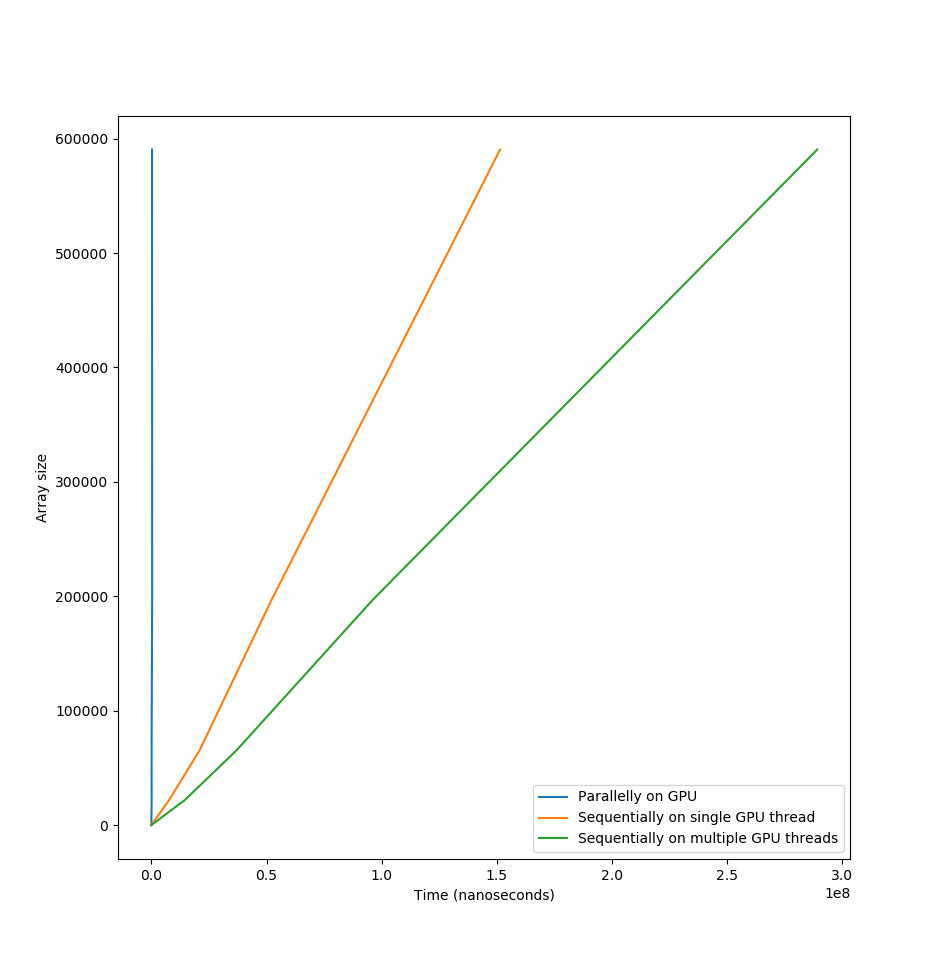
\includegraphics[scale=0.5]{Graphics/gpucomp.png}\hspace*{\fill}
\caption{Comparing performance of sequential and parallel GPU algorithms}
\end{figure}
Similar to the previous plot, we can see that our implementation of the given CPU algorithm to run parallely on the GPU is much faster than the sequential algorithms on the GPU. This gives us an inclination that our implementation is correct and gives a speedup over the sequential algorithm when executed on the same hardware (GPU in our test machine in this case)\footnote{We used an Nvidia GeForce 1070 Max Q for our tests}.

\begin{figure}[H]
\hfill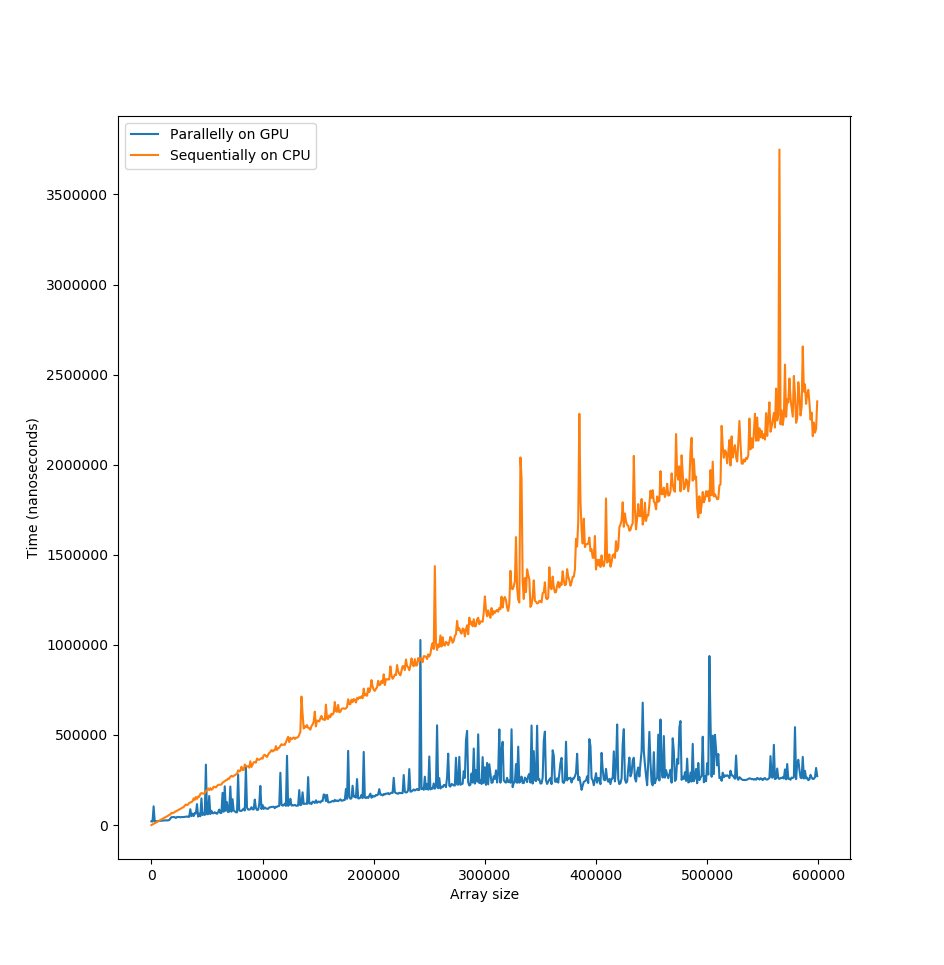
\includegraphics[scale=0.5]{Graphics/gpuvcpu.png}\hspace*{\fill}
\caption{Comparing parallelized GPU performance vs CPU performance}
\end{figure}
This is the most important result of the evaluation task. Here, we can clearly visualize that the parallel algorithm we designed to be executed on the GPU is much faster than the given sequential algorithm on the CPU.

\section{Appendix}
We have only demonstrated the relevant CUDA kernels and not the surrounding code or main functions which are required to execute the kernels. The entire collection of complete code samples can be found in the GitHub repository.\par
In our full sample code which we have used for benchmarking, we have used 2 header files which includes helper functions to facilitate CUDA error checking in our code - \textit{helper\_cuda.h} and \textit{helper\_string.h}. Both of these helper header files are included in the NVIDIA CUDA SDK under the \textit{samples/inc/} folder. In the Awkward Array production code we might use the same CUDA error checking header files or we might decide to write our own CUDA error checking code.

\end{document}
